\documentclass{standalone}
\usepackage{pgf-umlcd}
\begin{document}
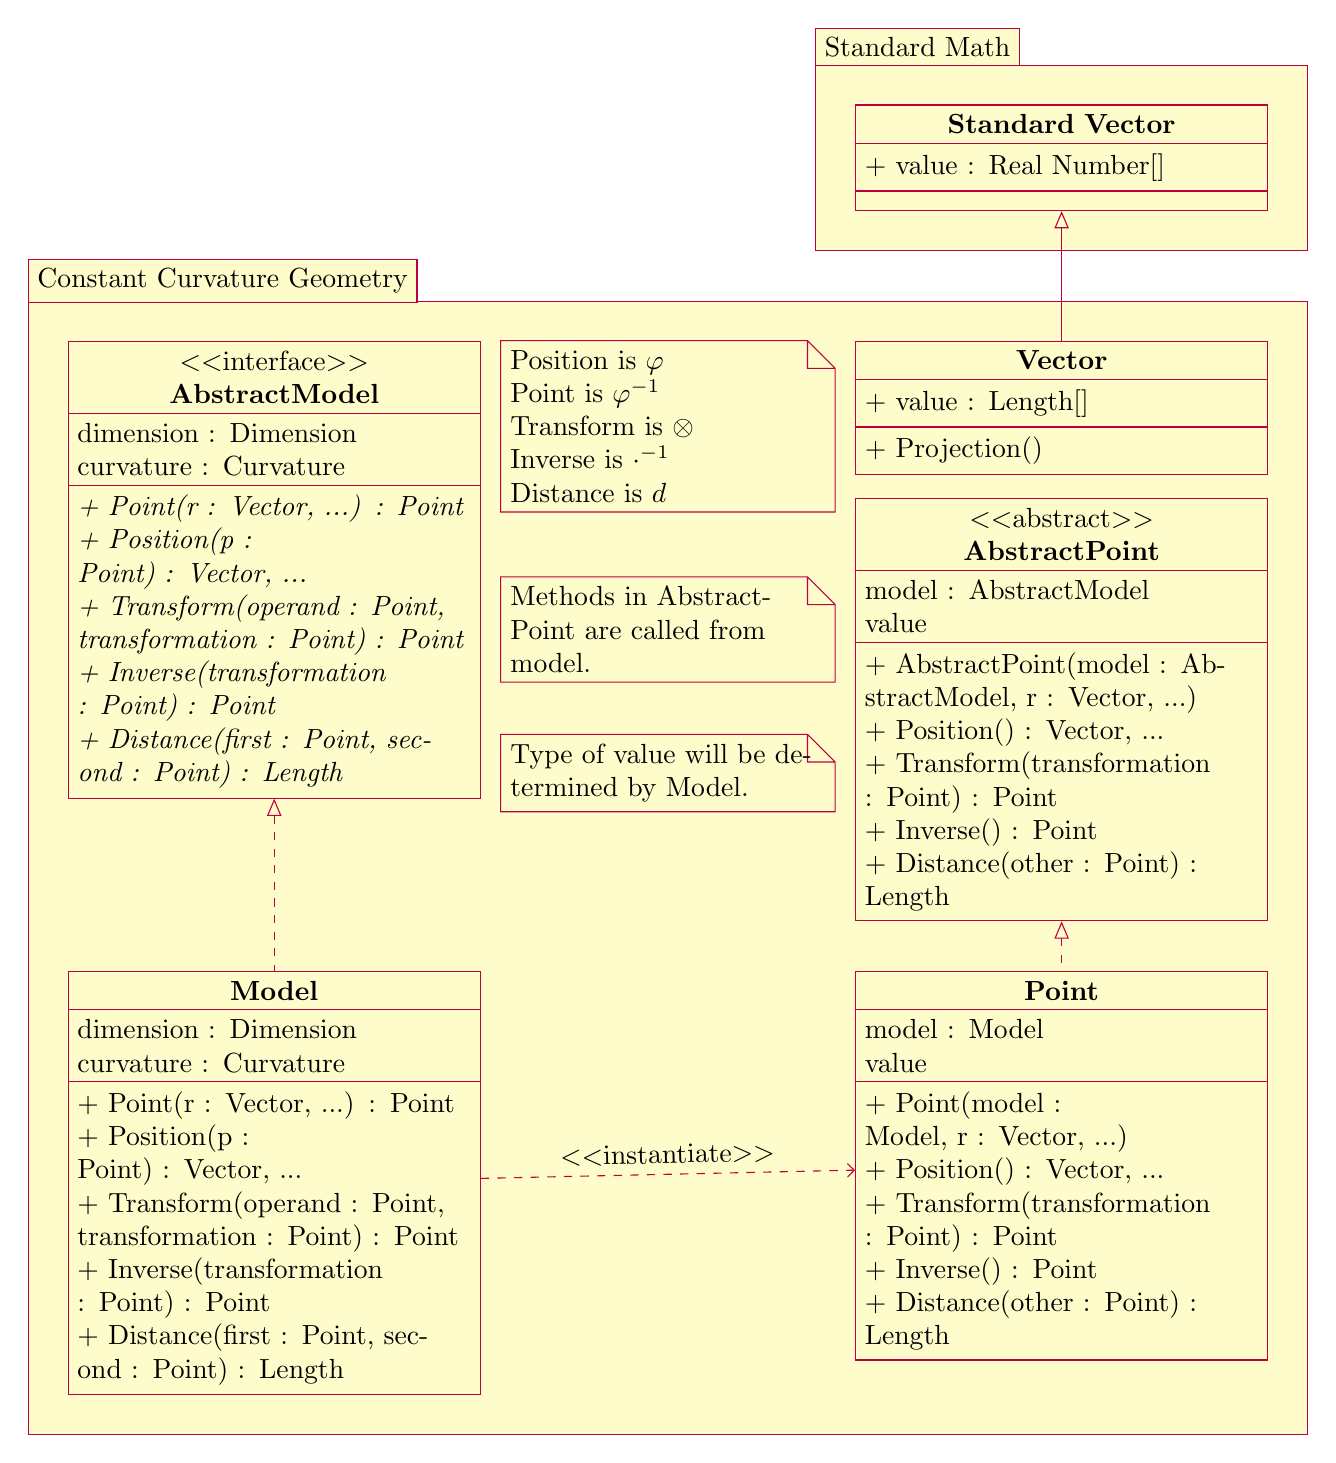
\begin{tikzpicture}
    \begin{package}{Standard Math}
        \begin{class}{Standard Vector}{10,0}
            \attribute{+ value : Real Number[]}
        \end{class}
    \end{package}
    \begin{package}{Constant Curvature Geometry}
        \begin{class}{Vector}{10,-3}
            \inherit{Standard Vector}
            \attribute{+ value : Length[]}
            \operation{+ Projection()}
        \end{class}
        \begin{interface}{AbstractModel}{0,-3}
            \attribute{dimension : Dimension}
            \attribute{curvature : Curvature}
            \operation[0]{+ Point(r : Vector, ...) : Point}
            \operation[0]{+ Position(p : Point) : Vector, ...}
            \operation[0]{+ Transform(operand : Point, transformation : Point) : Point}
            \operation[0]{+ Inverse(transformation : Point) : Point}
            \operation[0]{+ Distance(first : Point, second : Point) : Length}
        \end{interface}
        \begin{abstractclass}{AbstractPoint}{10,-5}
            \attribute{model : AbstractModel}
            \attribute{value}
            \operation{+ AbstractPoint(model : AbstractModel, r : Vector, ...)}
            \operation{+ Position() : Vector, ...}
            \operation{+ Transform(transformation : Point) : Point}
            \operation{+ Inverse() : Point}
            \operation{+ Distance(other : Point) : Length}
        \end{abstractclass}

        \umlnote (note) at (5, -3) {
            Position is $\varphi$ \\
            Point is $\varphi^{-1}$ \\
            Transform is $\otimes$ \\
            Inverse is $\cdot^{-1}$ \\
            Distance is $d$ \\
        };
        \umlnote (note) at (5, -6) {
            Methods in AbstractPoint are called from model.
        };
        \umlnote (note) at (5, -8) {
            Type of value will be determined by Model.
        };
        \begin{class}{Model}{0,-11}
            \implement{AbstractModel}
            \attribute{dimension : Dimension}
            \attribute{curvature : Curvature}
            \operation{+ Point(r : Vector, ...) : Point}
            \operation{+ Position(p : Point) : Vector, ...}
            \operation{+ Transform(operand : Point, transformation : Point) : Point}
            \operation{+ Inverse(transformation : Point) : Point}
            \operation{+ Distance(first : Point, second : Point) : Length}
        \end{class}
        \begin{class}{Point}{10,-11}
            \implement{AbstractPoint}
            \attribute{model : Model}
            \attribute{value}
            \operation{+ Point(model : Model, r : Vector, ...)}
            \operation{+ Position() : Vector, ...}
            \operation{+ Transform(transformation : Point) : Point}
            \operation{+ Inverse() : Point}
            \operation{+ Distance(other : Point) : Length}
        \end{class}
        \draw[umlcd style dashed line, ->] (Model) --node[above, sloped, black]{$<<$instantiate$>>$}(Point);
    \end{package}
\end{tikzpicture}
\end{document}